\documentclass[review]{elsarticle}

\usepackage{lineno,hyperref}
\modulolinenumbers[5]

\journal{Journal of Computers and Fluids}

%% `Elsevier LaTeX' style
\bibliographystyle{elsarticle-num}
\usepackage{caption}
\usepackage{subcaption}
\usepackage{amsmath}
%%%%%%%%%%%%%%%%%%%%%%%

\begin{document}

\begin{frontmatter}

\title{Data-Driven Multi-grid Solver for Accelerated \\ Pressure Projection}

%% Group authors per affiliation:
\author{Gabriel D Weymouth}
\address{Engineering and Physical Sciences, University of Southampton, Southampton, UK}
\address{Data-Centric Engineering, Alan Turing Institute, London, UK}
\ead[url]{https://weymouth.github.io/}

\begin{abstract}
Pressure projection is the single most computationally expensive step in an unsteady incompressible fluid simulation. This work discusses the potential of data-driven methods to accelerate the approximate solution of the Poisson equation at the heart of pressure projection, linking Multi-grid methods to convolutional encoder-decoder networks. Required to maintain linearity in pressure, the best option for data-driven acceleration is in the smoothing step. Using automatic differentiation, a high-speed parameterized smoother is developed which accelerates classic Multi-grid methods by 66-185\% on eleven 2D and 3D benchmarks with no loss of accuracy. The tuned parameters are found to transfer nearly 100\% effectiveness as the resolution is increased, providing a robust approach for accelerated pressure projection of general flows.
\end{abstract}

\begin{keyword}
pressure projection, linear algebra, data-driven
\end{keyword}

\end{frontmatter}

\section{Introduction}

Pressure projection is a bottleneck in high-speed unsteady incompressible flow solvers. Constructing approximate solutions the discrete pressure Poisson system is the most expensive part of each time-step as the elliptic equation requires communication throughout the computational domain instead of being confined to a local characteristic. As such, the proportional cost only grows in massively parallel simulations due to the required communication across processes. Methods such as artificial-compressibility \cite{he2002comparison}, smooth-particle-hydrodynamics \cite{kiara2013sph}, and particle-in-cell \cite{jiang2017angular} attempt to side-step this computational cost by modelling or otherwise under-resolving the pressure evolution compared to the fluid's momentum. However, these approaches lead to significant errors in pressure forces, thereby making them unsuitable for many applications or requiring explicit pressure corrections, \cite{kiara2013sph}.

Recent advances in data-driven acceleration of flow solvers have mainly focused on data-assimilation methods and data-driven turbulence closures. Data-assimilation methods typically avoid the expensive pressure projection step entirely, focusing on applications where time-accurate pressure forces are not important \cite{asch2016data}. Deep learning closures for Large Eddy Simulation (LES) \cite{BECK2019108910,maulik_san_rasheed_vedula_2019}, Unsteady Reynolds Averaged Navier-Stokes (unRANS) \cite{ling_kurzawski_templeton_2016}, and even Spanwise Averaged Navier-Stokes (SANS) \cite{font2021deep} simulations have seen growing success and are capable of accurate force prediction. However, none of these examples have accelerated the project step itself.

\begin{figure}
    \caption{Sketch of a Convolutional Neural Networks (CNN) and/or a Multi-grid V-cycle.}
    \label{fig:multigrid}
\end{figure}

Many of these turbulence closures as well as other fluids applications such as super-resolution \cite{ferdian20204dflownet,liu2020deep} and full field regression models \cite{duru2021cnnfoil,bhatnagar2019prediction} are based on Convolutional Neural Networks (CNN) and encoder-decoder architectures. CNNs have inherent translational symmetry and encoder-decoder architectures reduce the number of variables before expanding again, Figure \ref{fig:multigrid}, both of which help constrain learning capacity and generalize the trained networks to unseen prediction cases. 

A few studies have applied machine-learning to accelerate the critical projection step itself \cite{ozbay2021poisson,Xiao2020,ajuria2020}. All of these approaches use CNNs to predict the pressure field given the projection source term on a uniform grid, meaning they are limited to cases without internal solid geometries. While \cite{ozbay2021poisson} uses a decomposition to handle different \textit{domain} boundary conditions and grid aspect ratios in 2D and sees a significant speed-up over traditional Multi-grid methods, the results are still somewhat qualitative, with pressure errors greater than 10\% throughout much of the domain.

The primary insight of this paper is that Multi-grid methods are \textit{already} convolutional encoder-decoder networks with optimal $O(N\log N)$ scaling, prime for data-driven acceleration without any loss of accuracy in the resulting pressure field. This work develops an accurate data-driven projection method which outperforms classic Multi-grid on eleven 2D and 3D benchmarks including those with immersed solid boundaries. Moreover, since the new approach is linear in the pressure and the nonlinear dependence on the matrix coefficients are scale-invariant, the data-optimized parameters generalize extremely well to new flows and simulation resolutions.

\section{Linear System Description}

The discrete Poisson equation in the projection step is defined as
\begin{equation}\label{eq:axb}
    A x = b
\end{equation}
where $x$ is the desired pressure field vector, $b$ is the source term (proportional to the divergence of the velocity field to be projected), and $A$ is the Poisson matrix. For conservative Poisson equations, $A$ is symmetric, has zero-sum rows and columns, is negative semi-definite, and has a single zero eigenvalue. The matrix is also extremely sparse. While the solution vector size $N$ may easily be $10^6-10^8$, a second-order scheme on structured grids in $M$ dimensions result in only $M$ non-zero sub-diagonals.

Iterative methods solve equation \ref{eq:axb} by updating an approximate solution $x^k$ to a new solution $x^{k+1}$ with reduced error. As the problem is linear, the equation for the update $\epsilon$ is simply
\begin{equation}\label{eq:aer} 
    A \epsilon^k = r^k \equiv b - Ax^k
\end{equation}
where $r$ is the residual. In practise, only an approximate solution for $\epsilon$ is obtained, after which the solution and residual are incremented
\begin{equation}\label{eq:increment}
    x^{k+1} = x^k+\epsilon^k, \quad r^{k+1} = r^k-A\epsilon^k.
\end{equation}
This process is iterated until the residual is reduced sufficiently, the required tolerance level being highly dependant on the application.

Multi-grid (MG) methods are among the fastest iterative solution approaches for variable coefficient discrete pressure Poisson equations because the MG operator is effectively a \textit{linear} convolutional encoder-decoder network, Figure \ref{fig:multigrid}. The system is preconditioned before the residual is restricted down to a reduced-size problem and the correction is prolongated back up. 
% \begin{equation}
%     r_c = R r \quad\rightarrow\quad A_c \epsilon_c = r_c \quad\rightarrow\quad \epsilon = P \epsilon_c
% \end{equation}
% where $R$ is the $N_c \times N$ restriction operator, $P$ is the $N \times N_c$ prolongation operator 
The restriction-solve-prolongation process, a V-cycle, distributes the residual throughout the domain, which enables simple and relatively fast stationary methods such as Gauss-Sidel or Successive Over Relation (SOR) to smooth the local error in the projected solution. The MG architecture proceeds recursively on the reduced-size problems until they are small enough to be solved directly, resulting in $O(N\log N)$ computational cost overall. The V-cycle can be repeated until convergence or used as an efficient preconditioner for another iterative solver such as Conjugate Gradient. 

\section{Data-driven Accelerated Projection Method}

As \textit{any} element of the residual of the elliptic Poisson system potentially influences \textit{every} element of the update, $O(N\log N)$ is the best possible solution time scaling. However, data-driven methods can still be used to accelerate pressure projection by speeding-up and increasing the residual reduction of each V-cycle iteration.

The linearity of equation \ref{eq:aer} is a critical property which the data-driven method must maintain. Not only will this increase generality, but a nonlinear method could not be used iteratively since the modes of the residual will change as the solver converges. However, this linearity is only with respect to the update and residual fields. The operators of the MG method can all potentially be made into parameterized nonlinear functions of $A$, embedding information about the discrete problem and boundary conditions. 

Which MG operation is the best candidate for such an approach? The prolongation operator (and its transpose restriction operator) is not inherently a function of $A$, and while related super-resolution operators have seen use in the literature, these are nonlinear functions of the field. The precondition operator is an option, but a simple Jacobi preconditioner
\begin{equation}
    \epsilon = D^{-1}r
\end{equation}
where $D$ is the diagonal of $A$, is as fast as possible and is sufficient for the V-cycle to distribute the residual throughout the domain. Therefore, for the remainder of the paper we will focus on the smoother as the best candidate for parameterization, using a simple Jacobi preconditioner and uniform pooling/distribution for restriction/prolongation.

While more complex options are certainly possible, this work uses a simple parameterized Jacobi-like smoother
\begin{equation}\label{eq:smooth}
    \epsilon = \tilde A^{-1}r
\end{equation}
where $\tilde A^{-1}=f(A\,|\theta)$ is an approximate matrix-inverse with the same sparsity as $A$ and parameter vector $\theta$. 
%The matrix $A$ is constant during the projection step (and often for an entire simulation), meaning $\tilde A^{-1}$ can be computed and stored ahead of time.
As with all stationary smoothers, equation \ref{eq:smooth} can be iterated with equation \ref{eq:increment} in an inner loop at each MG level. Unlike Gauss-Sidel or SOR smoothers, the matrix-vector multiplication smoother requires no back-propagation and so can be vectorized in serial or parallel implementations, offering a significant potential speed-up. 

There are few constraints on $\tilde A^{-1}$: it must have units of $A^{-1}$, and symmetry of $A$ implies the approximate inverse should also be symmetric. For simplicity, the diagonal and off-diagonal coefficients of $\tilde A^{-1}$ are constructed independently 
\begin{equation}\label{eq:approxinv}
    \tilde a^{-1}_{ii} = \frac{f_d(a_{ii}/s\,|\theta_d)}{a_{ii}} , \quad
    \tilde a^{-1}_{ij} = \frac{f_o(a_{ij}/s\,|\theta_o)}{a_{ii}+a_{jj}}
\end{equation}
where function inputs are scaled by the maximum off-diagonal $s=\max(A-D)$ and the outputs are scaled by the diagonal elements. Note a Jacobi smoother would use a diagonal function $f_d=1$ and off-diagonal function $f_o=0$. With the learning problem now reduced to two normalized single-variable functions, the specific choice of parameterization is not critical and a simple quadratic polynomial $f(a) = \sum_{p=0}^2 a^p \theta_p$ is chosen for $f_o$ and $f_d$. Using higher-order polynomials, splines, and interpolating kernels did not significantly change the results.

The parameterized smoother is optimized for a set of training data $X=\{A,x^k,b\}$. The loss function is simply the reduction in the norm of the residual after a V-cycle iteration $L = \log_{10}(|r^{k+1}| / |r^{k}|)$, which means that example pressure \textit{solutions} are not required. This loss is averaged over each iteration and each example in the data-set. The optimal parameters are defined as
\begin{equation}
    \hat\theta = \min_\theta L(\theta\, |X)
\end{equation}
and determined using Newton's method. The residual loss function is a highly nonlinear recursive function of the parameters, but automatic differentiation (AD) is used to determine the gradient $\nabla_\theta L$ and Hessian $H_{\theta\theta} L$ \cite{RevelsLubinPapamarkou2016}, avoiding inaccurate and potentially unstable finite differences.

The data-driven solver and all test cases presented in the following sections are implemented in Julia and available for reproduction \cite{bezanson2017julia,weymouth2021julia}.

\begin{figure}
    \centering
    \begin{subfigure}[b]{0.3\textwidth}
        \centering
        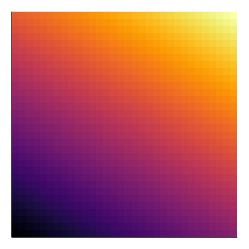
\includegraphics[width=\textwidth]{figures/2D-static.png}
        \caption{2D-static}
        \label{fig:2D-static}
    \end{subfigure}
    \begin{subfigure}[b]{0.3\textwidth}
        \centering
        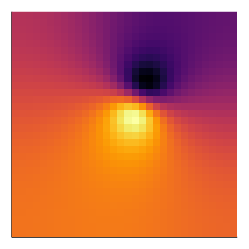
\includegraphics[width=\textwidth]{figures/2D-dipole.png}
        \caption{2D-dipole}
        \label{fig:2D-mu}
    \end{subfigure}
    \begin{subfigure}[b]{0.3\textwidth}
        \centering
        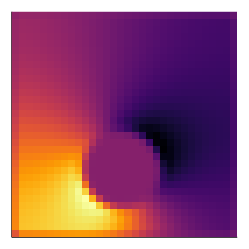
\includegraphics[width=\textwidth]{figures/2D-sphere.png}
        \caption{2D-sphere}
        \label{fig:2D-sphere}
    \end{subfigure}
    \caption{Sample solutions from the data-sets of three of the six synthetic cases.}
    \label{fig:synthetic cases}
\end{figure}
\begin{figure}
    \centering
    \begin{subfigure}[b]{0.47\textwidth}
        \centering
        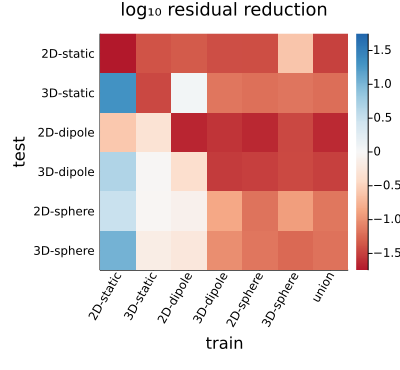
\includegraphics[width=\textwidth]{figures/crossloss.png}
        \caption{single-cycle residual reduction}
        \label{fig:cross plot}
    \end{subfigure}
    \hfill
    \begin{subfigure}[b]{0.47\textwidth}
        \centering
        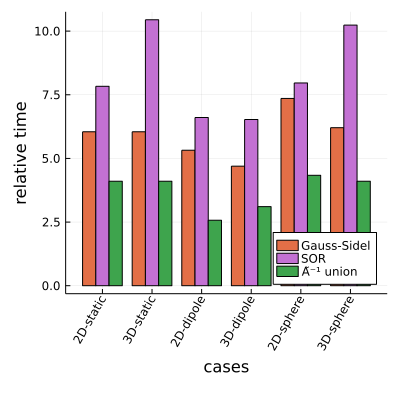
\includegraphics[width=\textwidth]{figures/synthetic_timing.png}
        \caption{solver time}
        \label{fig:synthetic time}
    \end{subfigure}
    \caption{a) Residual reduction over a single Multi-grid V-cycle on the `test' cases after tuning using the `train' case. Training case `union' refers to the smoother trained on all of the synthetic cases. (b) Time to reduce pressure residual by $10^{-3}$ for classical and parameterized smoothers on each synthetic case. Time is relative to the time of a single V-cycle using the Jacobi smoother.}
    \label{fig:synthetic results}
\end{figure}

\section{Synthetic Discrete Poisson System Results}

A set of six synthetic projection cases were constructed to establish the characteristics of the parameterized smoother. The three 2D cases are shown in Figure~\ref{fig:synthetic cases}, and each has a matching 3D case. The `static' cases have a hydrostatic gradient throughout the domain, with the direction and magnitude randomized. The `dipole' and `sphere' cases have a randomized dipole/sphere within a quiescent flow. All cases are initialized with $x^0=0$.
%, and all cases feature initially localized residuals; i.e. $r^0\ne0$ only in a fraction of the cells, but $x$ must be updated throughout the domain, starkly illustrating the elliptic nature of the projection step.
Neumann boundary conditions are applied on all boundaries, including the boundary of the immersed sphere, through adjustment of the $A$ matrix coefficients which are otherwise uniform. 

Figure~\ref{fig:cross plot} characterizes the generalization of the parameterized smoother's residual reduction over a single V-cycle on 100 randomized `test' case examples after optimization using 100 examples of the `train' case. Each example uses a grid size of $n=32^M$ points ($N=32^2$ in 2D and $N=32^3$ in 3D) as testing with other resolutions found essentially no change in the performance. Two inner loops are used throughout to optimize residual reduction. As expected, the performance is best when testing and training on the same case, with a single V-cycle reducing the residual from $10^{-1.17}$ on the 2D-sphere case down to $10^{-1.58}$ on the 3D-box case. While the performance for the simplest cases generalizes poorly, the 2D-sphere smoother generalizes essentially as well as the `union' smoother trained on all of the data. 

Finally, the acceleration of the `union' data-driven smoother is evaluated on new example data of a different size, $n=64^M$ points. Figure~\ref{fig:synthetic time} shows the time to reduce the residual of each case by $10^{-3}$ relative to the time to run a single V-cycle using a Jacobi smoother. While a Jacobi smoother requires  hundreds or even thousands of V-cycles to converge, the Jacobi-like parameterized smoother is only around 30-50\% slower per V-cycle, and yet converges in only 1-3 V-cycles in all cases. This results in a 80-174\% speed-up (mean: 119\%) relative to optimized serial Gauss-Sidel and SOR smoothers. This speed-up will be even more favorable in parallel computation as the new smoother operates directly on the local residual without back-propagation, eliminating any additional communication.

\begin{figure}
    \centering
    \begin{subfigure}[b]{0.3\textwidth}
        \centering
        \caption{circle flow}
        \label{fig:circle}
    \end{subfigure}
    \begin{subfigure}[b]{0.3\textwidth}
        \centering
        \caption{Taylor-Green Vortex}
        \label{fig:TGV}
    \end{subfigure}
    \begin{subfigure}[b]{0.3\textwidth}
        \centering
        \caption{flapping wing}
        \label{fig:wing}
    \end{subfigure}
    % \begin{minipage}{0.47\textwidth}
        \begin{subfigure}{0.47\textwidth}
        \centering
        \caption{torus flow}
        \label{fig:donut}
        \end{subfigure}
        \hfill
        \begin{subfigure}{0.47\textwidth}
        \centering
        \caption{swimming shark}
        \label{fig:shark}
        \end{subfigure}
    % \end{minipage}
    \hfill
    % \begin{subfigure}[b]{0.47\textwidth}
    %     \centering
    %     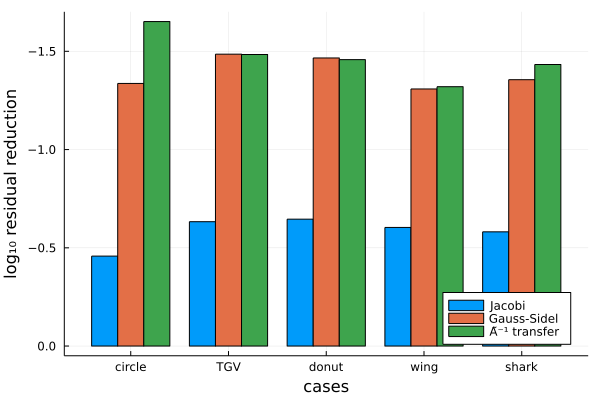
\includegraphics[width=\textwidth]{figures/compareloss.png}
    %     \caption{single-cycle residual reduction}
    %     \label{fig:simulation residual}
    % \end{subfigure}
    \caption{(a-e) Snapshots from the five flow simulation cases. The Taylor-Green Vortex and torus flow are 3D, the flapping wing is dynamic without a background flow and the swimming shark is a deforming geometry.}
    \label{fig:simulation cases}
\end{figure}

\section{Unsteady Incompressible Simulation Results}

Five unsteady incompressible simulation cases were used to further characterize the accelerated projection method, Figure \ref{fig:simulation cases}. All simulations use the same validated Cartesian-grid method \cite{maertens2015accurate} but feature significantly different physics, i.e. 2D and 3D simulations with and without background flows, immersed geometries, body motion, and body deformation.

\begin{figure}
    \centering
    \begin{subfigure}[b]{0.47\textwidth}
        \centering
        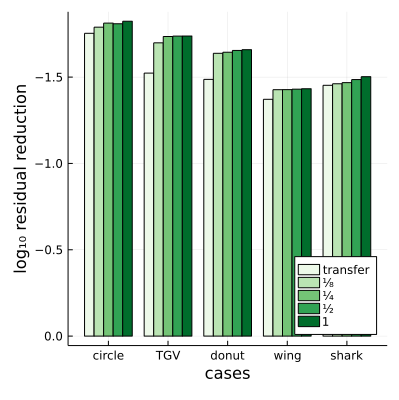
\includegraphics[width=\textwidth]{figures/scaleloss.png}
        \caption{single-cycle residual reduction}
        \label{fig:scaled loss}
    \end{subfigure}
    \hfill
    \begin{subfigure}[b]{0.47\textwidth}
        \centering
        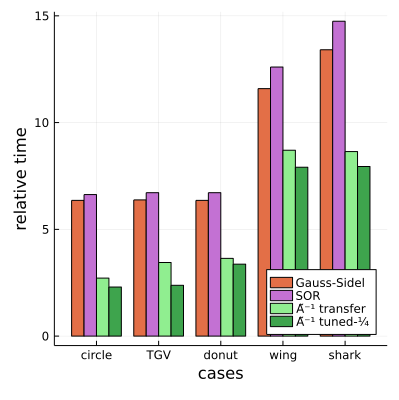
\includegraphics[width=\textwidth]{figures/crosscount.png}
        \caption{solver time}
        \label{fig:simulation time}
    \end{subfigure}
        \caption{(a) Residual reduction over a single Multi-grid V-cycle on the full-resolution case. The `transfer' smoother has been trained on the union of the synthetic data sets from Figure~\ref{fig:synthetic cases}. The $\frac 18, \frac 14, \frac 12$ smoothers have been trained on simulations with the indicated reduced resolution \textit{in each spacial and temporal dimension}. (b) Time to reduce pressure residual by $10^{-3}$ for classical and parameterized smoothers on each simulation case. Time is relative to the time of a single V-cycle using the Jacobi smoother.}
        \label{fig:tuned simulation}
\end{figure}

The parameterized smoother from the synthetic cases of the previous section is effective at reducing the residual on the unseen simulation cases, Figure \ref{fig:scaled loss}. This `transfer' smoother achieves 85-95\% of the residual reduction of a smoother optimized for each case. Even more promising is that training on reduced-size simulations closes that small gap almost completely. Training on a $1/4^\text{th}$-scale simulation is fast, requiring only $N_{1/4} = N/4^M$ points (N/16 in 2D and N/64 in 3D) and $\approx 1/4$ the number of time steps, while achieving 99-100\% of the residual reduction of training with full-scale data. Such an \textit{auto-tuning} approach enables a highly effective data-driven projection method to be developed for any simulation approach with very little overhead.

The relative speed-up of this approach is compared to classic MG methods and the transfer smoother in Figure \ref{fig:simulation time}. As with the synthetic cases of the previous section, the data-driven methods are much faster, with the auto-tuned approach accelerating the projection step by 66-120\%.

\begin{figure}
    \centering
    \begin{subfigure}[b]{0.47\textwidth}
        \centering
        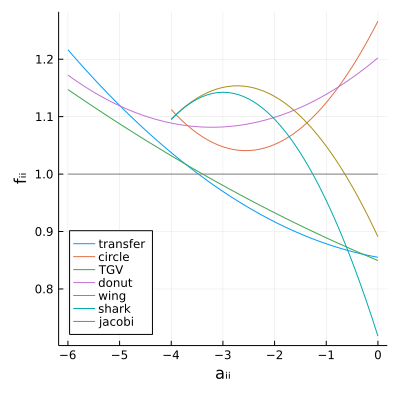
\includegraphics[width=\textwidth]{figures/diag_fun.png}
        \caption{diagonal functions}
    \end{subfigure}
    \hfill
    \begin{subfigure}[b]{0.47\textwidth}
        \centering
        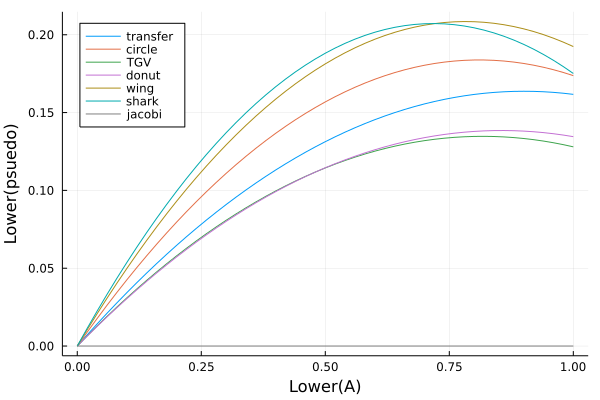
\includegraphics[width=\textwidth]{figures/lower_fun.png}
        \caption{off-diagonal functions}
    \end{subfigure}
        \caption{(a) Diagonal and (b) off-diagonal parameterized functions after optimization on each simulation case. The `transfer' smoother was tuned on the synthetic cases and `Jacobi' is shown for comparison.}
        \label{fig:tuned inverse}
\end{figure}

Finally, the parameterized $f_d,\,f_o$ functions used in the approximate inverse equation \ref{eq:approxinv} are shown in Figure \ref{fig:tuned inverse}. It is interesting to note that the diagonal functions are all somewhat centered on one and the off-diagonal values all have an essentially zero intercept as these are the values for the Jacobi smoother. We also note that the `wing' and `shark' cases produce parameterizations which are similar to each other but significantly different than the others cases. This is reasonable as dynamic and deforming geometries put unique burdens on the pressure projection step, as shown in the longer convergence times for these cases shown in Figure \ref{fig:simulation time}. Adopting a data-driven and auto-tuned approach enables these pressure-projection dominated cases to achieve significant accelerations.

\section{Conclusions}

This manuscript develops a successful data-driven method to accelerate the solution of discrete pressure Poisson systems found in incompressible flow simulations. Multi-grid methods are identified as linear convolutional encoder-decoder networks with optimal ($N\log N$) scaling, and the matrix coefficients are identified as the critical nonlinear input, not the projection source-term, embedding information such as boundary conditions. Mathematical constraints are used to further focus the learning capacity to a parameterized Jacobi-like Multi-grid smoother. This resulting data-driven MG solver is with 33\% of the minimum computational cost per V-cycle, and shown to outperform classic Gauss-Sidel and SOR smoothers by 66-185\% on eleven simulation cases. Because of the focused learning capacity, the generalization is excellent, enabling 90\% effective transfer learning from a synthetic data-set and essentially perfect transfer from reduced resolution simulations. 

The potential of machine learning and computer science advances to improve fluid dynamics is vast, but well-applied classical methods and constraints only helps to focus this effort. Wherever possible, this work has made the simplest choice in parameterization, leaving significant opportunities for future improvements. Many other flow solvers and linear systems are yet to be explored, and extensions to this basic data-driven approach could accelerate solutions for a wide array of discrete partial differential equations. 


\bibliography{mybibfile}

\end{document}